\documentclass[12pt]{article}
\usepackage{parskip}
\usepackage[slantedGreek]{mathpazo}
\usepackage{amsmath,amssymb,amsthm,amsfonts}
\usepackage[top=8pc,bottom=8pc,left=8pc,right=8pc]{geometry}
%\usepackage{ntheorem}

\usepackage{graphicx}
\usepackage{wrapfig}
\usepackage{epstopdf}
\usepackage{subcaption}
\usepackage{multirow}
\usepackage{nicefrac}

%% Please use the following statements for
%% managing the text and math fonts for your papers:
\usepackage{times}
%\usepackage[cmbold]{mathtime}
\usepackage{bm}

\usepackage{array}
\newcolumntype{L}[1]{>{\raggedright\let\newline\\\arraybackslash\hspace{0pt}}m{#1}}
\newcolumntype{C}[1]{>{\centering\let\newline\\\arraybackslash\hspace{0pt}}m{#1}}
\newcolumntype{R}[1]{>{\raggedleft\let\newline\\\arraybackslash\hspace{0pt}}m{#1}}

 \newcommand{\beginsupplement}{%
        \setcounter{equation}{0}
				\setcounter{page}{0}
				\setcounter{table}{0}
				\setcounter{section}{0}
				\setcounter{figure}{0}

			\numberwithin{table}{section}
			\renewcommand{\theequation}{S.\arabic{equation}}
			\renewcommand{\thesection}{S.\arabic{section}}
			\renewcommand{\thesubsection}{S.\arabic{section}.\arabic{subsection}}
			\renewcommand{\thepage}{S.\arabic{page}}
			\renewcommand{\thetable}{S.\arabic{table}}
			\renewcommand{\thefigure}{S.\arabic{figure}}
}
  
% this order is important
\RequirePackage[hyphens]{url}
\RequirePackage[colorlinks,citecolor=blue,urlcolor=blue]{hyperref}
\usepackage[authoryear]{natbib}

\usepackage[plain,noend]{algorithm2e}

% For compressing some space: 
\setlength{\textfloatsep}{10pt plus 1.0pt minus 2.0pt}
\setlength{\floatsep}{12.0pt plus 2.0pt minus 5.0pt}
\setlength{\intextsep}{12.0pt plus 2.0pt minus 5.0pt}
\setlength{\belowcaptionskip}{-2pt}

%\setlength{\textheight}{9in}
%\setlength{\textwidth}{6in}
%\setlength{\topmargin}{-36pt}
%\setlength{\oddsidemargin}{0pt}
%\setlength{\evensidemargin}{0pt}

%% Special shortcuts for us
\def\Polya{P{\'o}lya}
\def\CS{Cauchy-Schl\"omilch}
\def\PG{P{\'o}lya-Gamma}

\usepackage{array}
%
% Math commands by Thomas Minka 
%
% Revised by Jyotishka Datta & Brandon Willard
% Acknowledgement: JD received this from Prof. Alan Qi.
%


%% Special shortcuts for us
\def\Polya{P{\'o}lya}
\def\CS{Cauchy-Schl\"omilch}
\def\PG{P{\'o}lya-Gamma}

%\setlength{\textfloatsep}{10pt plus 1.0pt minus 2.0pt}
%\setlength{\floatsep}{12.0pt plus 2.0pt minus 5.0pt}
%\setlength{\intextsep}{12.0pt plus 2.0pt minus 5.0pt}
%\setlength{\belowcaptionskip}{-2pt}

%\def\distrib{\mathrel{\ooalign{%
%  \raisebox{0.75\height}{{\small{ind}}}\cr\hidewidth$\sim$\hidewidth\cr}}}
%  
\newcommand{\var}{{\rm var}}
\newcommand{\Tr}{^{\rm T}}
\newcommand{\rmlog}{\rm log}
\newcommand{\vtrans}[2]{{#1}^{(#2)}}
\newcommand{\kron}{\otimes}
\newcommand{\schur}[2]{({#1} | {#2})}
\newcommand{\schurdet}[2]{\left| ({#1} | {#2}) \right|}
\newcommand{\had}{\circ}
\newcommand{\diag}{{\rm diag}}
\newcommand{\invdiag}{\diag^{-1}}
\newcommand{\rank}{{\rm rank}}
% careful: ``null'' is already a latex command
\newcommand{\nullsp}{{\rm null}}
\newcommand{\tr}{{\rm tr}}
\renewcommand{\vec}{{\rm vec}}
\newcommand{\vech}{{\rm vech}}
\renewcommand{\det}[1]{\left| #1 \right|}
\newcommand{\pdet}[1]{\left| #1 \right|_{+}}
\newcommand{\pinv}[1]{#1^{+}}
\newcommand{\erf}{{\rm erf}}
\newcommand{\hypergeom}[2]{{}_{#1}F_{#2}}

% boldface characters
\renewcommand{\a}{{\bf a}}
\renewcommand{\b}{{\bf b}}
\renewcommand{\c}{{\bf c}}
\renewcommand{\d}{{\rm d}}  % for derivatives
\newcommand{\e}{{\rm e}} % for exponentials
\newcommand{\f}{{\bf f}}
\newcommand{\g}{{\bf g}}
\newcommand{\h}{{\bf h}}
%\newcommand{\k}{{\bf k}}
% in Latex2e this must be renewcommand
\renewcommand{\k}{{\bf k}}
\newcommand{\m}{{\bf m}}
\newcommand{\n}{{\bf n}}
%\renewcommand{\o}{{\bf o}}
\newcommand{\p}{{\bf p}}
%\newcommand{\q}{{\bf q}}
\renewcommand{\r}{{\bf r}}
\newcommand{\s}{{\bf s}}
\renewcommand{\t}{{\bf t}}
\renewcommand{\u}{{\bf u}}
\renewcommand{\v}{{\bf v}}
\newcommand{\w}{{\bf w}}
%\newcommand{\x}{{\bf x}}
\newcommand{\y}{{\bf y}}
%\newcommand{\z}{{\bf z}}
\newcommand{\A}{{\bf A}}
\newcommand{\B}{{\bf B}}
%\newcommand{\C}{{\bf C}}
\newcommand{\D}{{\bf D}}
\newcommand{\E}{{\bf E}}
\newcommand{\F}{{\bf F}}
%\newcommand{\G}{{\bf G}}
\renewcommand{\H}{{\bf H}}
\newcommand{\I}{{\bf I}}
\newcommand{\J}{{\bf J}}
\newcommand{\K}{{\bf K}}
\renewcommand{\L}{{\bf L}}
\newcommand{\M}{{\bf M}}
%\newcommand{\N}{{\bf N}}
\renewcommand{\O}{{\bf O}}
\renewcommand{\P}{{\bf P}}
\newcommand{\Q}{{\bf Q}}
\newcommand{\R}{{\bf R}}
%\renewcommand{\S}{{\bf S}}
\newcommand{\T}{{\rm T}}
%\newcommand{\U}{{\bf U}}
\newcommand{\V}{{\bf V}}
\newcommand{\W}{{\bf W}}
\newcommand{\X}{{\bf X}}
\newcommand{\Y}{{\bf Y}}
\newcommand{\Z}{{\bf Z}}

% this is for latex 2.09
% unfortunately, the result is slanted - use Latex2e instead
%\newcommand{\bfLambda}{\mbox{\boldmath$\Lambda$}}
% this is for Latex2e
\newcommand{\bfLambda}{\boldsymbol{\Lambda}}

% Yuan Qi's boldsymbol
\newcommand{\bsigma}{\boldsymbol{\sigma}}
\newcommand{\balpha}{\boldsymbol{\alpha}}
\newcommand{\bpsi}{\boldsymbol{\psi}}
\newcommand{\bphi}{\boldsymbol{\phi}}
\newcommand{\bbeta}{\boldsymbol{\beta}}
%\newcommand{\Beta}{\boldsymbol{\eta}}
\newcommand{\btau}{\boldsymbol{\tau}}
\newcommand{\bvarphi}{\boldsymbol{\varphi}}
\newcommand{\bzeta}{\boldsymbol{\zeta}}
\newcommand{\bnabla}{\boldsymbol{\nabla}}
\newcommand{\blambda}{\boldsymbol{\lambda}}
\newcommand{\bLambda}{\mathbf{\Lambda}}

\newcommand{\btheta}{\boldsymbol{\theta}}
\newcommand{\bpi}{\boldsymbol{\pi}}
\newcommand{\bPi}{\boldsymbol{\Pi}}
\newcommand{\bxi}{\boldsymbol{\xi}}
\newcommand{\bSigma}{\boldsymbol{\Sigma}}

\newcommand{\bgamma}{\mathbf{\gamma}}
\newcommand{\bGamma}{\mathbf{\Gamma}}

\newcommand{\bmu}{\boldsymbol{\mu}}
\newcommand{\bnu}{\boldsymbol{\nu}}
\newcommand{\bPsi}{\mathbf{\Psi}}
\newcommand{\bepsilon}{\boldsymbol{\epsilon}}
\newcommand{\bOmega}{\boldsymbol{\Omega}}

\newcommand{\1}{{\bf 1}}
\newcommand{\0}{{\bf 0}}

%\newcommand{\comment}[1]{}

\newcommand{\bs}{\backslash}
\newcommand{\ben}{\begin{enumerate}}
\newcommand{\een}{\end{enumerate}}
\newcommand{\beq}{\begin{equation}}
\newcommand{\eeq}{\end{equation}}
\newcommand{\bde}{\begin{description}}
\newcommand{\ede}{\end{description}}

\newcommand{\notS}{{\backslash S}}
\newcommand{\nots}{{\backslash s}}
\newcommand{\noti}{{\backslash i}}
\newcommand{\notj}{{\backslash j}}
\newcommand{\nott}{\backslash t}
\newcommand{\notone}{{\backslash 1}}
\newcommand{\nottp}{\backslash t+1}
% \newcommand{\notz}{\backslash z}

\newcommand{\notk}{{^{\backslash k}}}
%\newcommand{\noti}{{^{\backslash i}}}
\newcommand{\notij}{{^{\backslash i,j}}}
\newcommand{\notg}{{^{\backslash g}}}
\newcommand{\wnoti}{{_{\w}^{\backslash i}}}
\newcommand{\wnotg}{{_{\w}^{\backslash g}}}
\newcommand{\vnotij}{{_{\v}^{\backslash i,j}}}
\newcommand{\vnotg}{{_{\v}^{\backslash g}}}
\newcommand{\half}{\frac{1}{2}}
\newcommand{\quart}{\frac{1}{4}}
\newcommand{\msgb}{m_{t \leftarrow t+1}}
\newcommand{\msgf}{m_{t \rightarrow t+1}}
\newcommand{\msgfp}{m_{t-1 \rightarrow t}}

\newcommand{\proj}[1]{{\rm proj}\negmedspace\left[#1\right]}
\newcommand{\argmin}{\operatornamewithlimits{argmin}}
\newcommand{\argmax}{\operatornamewithlimits{argmax}}

\newcommand{\dif}{\mathrm{d}}
\newcommand{\abs}[1]{\lvert#1\rvert}
\newcommand{\norm}[1]{\lVert#1\rVert}
\newcommand{\vectornorm}[1]{\left|\left|#1\right|\right|}

\newcommand{\NormRV}{\mathcal{N}}
\newcommand{\InvGaussRV}{\mathcal{IG}}
\newcommand{\CauchyRV}{\mathcal{C}}
\newcommand{\GammaRV}{\mathcal{G}}
\newcommand{\UnifRV}{\mathcal{U}}

\newcommand{\bx}{{\bf x}}
\newcommand{\ba}{{\bf a}}
\newcommand{\bb}{{\bf b}}
\newcommand{\bc}{{\bf c}}
\newcommand{\bd}{{\bf d}}
\newcommand{\bX}{{\bf X}}
\newcommand{\by}{{\bf y}}
\newcommand{\dd}[2]{\frac{\partial #1}{\partial #2}}
\newcommand{\lhat}[1][i]{\hat\lambda_{#1}^{-1(g)}}
\newcommand{\what}[1][j]{\hat\omega_{#1}^{-1(g)}}
\newcommand{\bone}{{\bf 1}}
\newcommand{\Li}{\hat\Lambda^{-1(g)}}
\newcommand{\Oi}{\hat\Omega^{-1(g)}}
\newcommand{\iid}{\stackrel{\mathrm{iid}}{\sim}}
\newcommand{\iidp}{\stackrel{\mathrm{P}}{=}}
\newcommand{\iidd}{\stackrel{\mathrm{D}}{=}}
\newcommand{\defeq}{\operatorname{:=}}

% the last {} is a hack for double subscript errors
\newcommand{\estHsp}{\ensuremath{{\hat{\theta}}_{HS+}}{}}
\newcommand{\estHs}{\ensuremath{{\hat{\theta}}_{HS}}{}}
\newcommand{\estJs}{\ensuremath{{\hat{\theta}}_{JS}}{}}
\newcommand{\MSE}{\mathrm{MSE}}

%% INTEGRALS 

\newcommand{\intreal}{\int_{-\infty}^{\infty}}
\newcommand{\intpos}{\int_{0}^{\infty}}
\newcommand{\intunit}{\int_{0}^{1}}


%\newtheorem{theorem}{THEOREM}
%\numberwithin{theorem}{section}
%\newtheorem{Proof}{PROOF}
%\newtheorem{Def}{DEFINITION}
%\numberwithin{Def}{section}
%\newtheorem{remark}{REMARK}
%\numberwithin{remark}{section}
%\newtheorem{Qes}{Question}
%\newtheorem{proposition}{PROPOSITION}
%\numberwithin{proposition}{section}
%\newtheorem{lemma}{LEMMA}
%\numberwithin{lemma}{section}
%\newtheorem{Cor}{COROLLARY}
%\numberwithin{Cor}{section}
%\newtheorem{Exa}{Example}
%\newtheorem{Eq}{Equation}
%\newtheorem{assn}{ASSUMPTION}
%\newtheorem{result}[theorem]{Result}
%\newtheorem{result}[theorem]{RESULT}

\newtheoremstyle{slplain}% name
  {1\baselineskip\@plus.2\baselineskip\@minus.2\baselineskip}% Space above
  {.5\baselineskip\@plus.2\baselineskip\@minus.2\baselineskip}% Space below
  {\slshape}% Body font
  {}%Indent amount (empty = no indent, \parindent = para indent)
  {\bfseries}%  Thm head font
  {.}%       Punctuation after thm head
  { }%      Space after thm head: " " = normal interword space;
        %       \newline = linebreak
  {}%       Thm head spec


\theoremstyle{slplain}

\newtheorem{theorem}{Theorem}
\newtheorem{acknowledgement}[theorem]{Acknowledgement}
%\newtheorem{algorithm}[theorem]{Algorithm}
\newtheorem{axiom}[theorem]{Axiom}
\newtheorem{case}[theorem]{Case}
\newtheorem{claim}[theorem]{Claim}
\newtheorem{conclusion}[theorem]{Conclusion}
\newtheorem{condition}[theorem]{Condition}
\newtheorem{conjecture}[theorem]{Conjecture}
\newtheorem{corollary}[theorem]{Corollary}
\newtheorem{criterion}[theorem]{Criterion}
\newtheorem{definition}[theorem]{Definition}
\newtheorem{example}[theorem]{Example}
\newtheorem{exercise}[theorem]{Exercise}
\newtheorem{lemma}[theorem]{Lemma}
\newtheorem{notation}[theorem]{Notation}
\newtheorem{problem}[theorem]{Problem}
\newtheorem{proposition}[theorem]{Proposition}
\newtheorem{remark}[theorem]{Remark}
\newtheorem{solution}[theorem]{Solution}
\newtheorem{summary}[theorem]{Summary}

\usepackage{booktabs,array}
\def\Midrule{\midrule[\heavyrulewidth]}
\newcount\rowc

%
%\makeatletter
%\def\ttabular{%
%\hbox\bgroup
%\let\\\cr
%\def\rulea{\ifnum\rowc=\@ne \hrule height 1.0pt \fi}
%\def\ruleb{
%\ifnum\rowc=1\hrule height 1.0pt  \else
%%\ifnum\rowc=3\hrule height 0.0pt%\heavyrulewidth 
%\ifnum\rowc= 3  \hrule height 0.5pt \else%\heavyrulewidth 
%\ifnum\rowc= 5  \hrule height 0.5pt \else%\heavyrulewidth 
%\ifnum\rowc= 7  \hrule height 0.5pt \else%\heavyrulewidth 
%\ifnum\rowc= 9  \hrule height 0.5pt \else%\heavyrulewidth 
%\ifnum\rowc= 11  \hrule height 0.5pt %\heavyrulewidth 
  %\else \hrule height 0pt%\lightrulewidth
%\fi\fi\fi\fi\fi\fi}
%\valign\bgroup
%\global\rowc\@ne
%\rulea
%\hbox to 7em{\strut \hfill##\hfill}%
%\ruleb
%&&%
%\global\advance\rowc\@ne
%\hbox to 7em{\strut\hfill##\hfill}%
%\ruleb
%\cr}
%\def\endttabular{%
%\crcr\egroup\egroup}
%

%\linespread{1.1}

\begin{document}

%% The left and right page headers are defined here:
\markboth{Bhadra, Datta, Polson, and Willard}{Bayesian $\sqrt{\text{Lasso}}$ }

% Here are the title, author names and addresses
\title{Bayesian $\sqrt{\text{Lasso}}$}

\author{Anindya Bhadra  \footnote{{\em Address:} 250 N. University St., West Lafayette, IN 47907, email: bhadra@purdue.edu.} \\ Purdue University \\ Department of Statistics 
\and Jyotishka Datta  \footnote{{\em Address:} Department of Mathematical Sciences, SCEN 309, 1 University of Arkansas, Fayetteville, AR, 72701, email: jd033@uark.edu.}\\ University of Arkansas \\ Department of Mathematical Sciences 
\and Nicholas G. Polson \footnote{{\em Address:} 5807 S. Woodlawn Ave., Chicago, IL 60637, email: ngp@chicagobooth.edu.} \\ University of Chicago \\ Booth School of
Business \and Brandon Willard \footnote{{\em Address:} 5807 S. Woodlawn Ave., Chicago, IL 60637, email: brandonwillard@gmail.com.} \\ University of Chicago \\ Booth School of
Business}

\maketitle

%\begin{abstract}
%In this paper, we provide a new class of sparsity priors in the global-local scale mixture family that has a higher spike near the origin and heavier tails compared to the other priors. These new shrinkage priors have the advantage of a closed-form prior density and penalty term as well as analytical tractability of the marginal distributions. These priors also enjoy the optimality properties shared by the horseshoe prior \cite{carvalho2010horseshoe} and its sharpened version, the horseshoe+ prior \cite{bhadra2015horseshoe+}, both in theory and in applications. 
%\end{abstract}

\section{Introduction}

Regularized methods have become widely popular as a inferential tool in high-dimensional data, owing to the popularity of Lasso \citep{tibshirani96} and many of its variants \citep{tibshirani2014praise}. Regularized methods prevent overfitting by controlling the bias-variance trade-off and are particularly useful for sparse learning, when the number of variables ($p$) exceed the number of observations ($n$). In the context of linear regression $Y = X \bbeta + \bepsilon$, a regularized estimate of $\bbeta$ is obtained by minimizing the penalized likelihood:
\begin{align}
\hat{\bbeta}_{\lambda^*}^{\text{pen}} & = \argmin_{\bbeta \in \Re^p} \{ \vectornorm{Y - X\bbeta}^2 + \lambda^* \Omega(\bbeta) \}, \label{eq:penalize} \\
  \text{where, } & \Omega(\bbeta) = \sum_{j=1}^{p} \omega(\beta_j) \text{ is a separable penalty}
\end{align}
The gold-standard for regularized method is Lasso that simultaneously performs estimation and model selection by constraining the $\ell_1$ norm of the underlying parameter vector, i.e. $\omega(\beta_j) = \abs{\beta_j}$. 
\beq
\hat{\bbeta}_{\lambda^*}^{\text{lasso}} = \argmin_{\bbeta \in \Re^p} \{ \vectornorm{Y - X\bbeta}^2 + \lambda^* \norm{\bbeta}_1 \} \label{eq:lasso}
\eeq

Lasso enjoys both computational efficiency, due to LARS \citep{efron_least_2004} and coordinate descent \citep{friedman_pathwise_2007}, as well as theoretical optimality properties \citep{buhlmann2011statistics}. \citet{bickel2009simultaneous} have shown that the Lasso estimator achieves near-orcale property in recovering the true $\bbeta_0$, under Gaussianity and certain design matrix conditions, up to a factor of $\sqrt{\log( 2 p)}$: yielding a $\sqrt{\log n}$ rate when $p$ grown polynomially as $n$. However, Lasso's performance in high-dimensional data is critically dependent on estimating the standard deviation $\sigma$ of the noise $\epsilon$, which remains a non-trivial problem in $p \gg n$ situation. The square-root Lasso, proposed by \cite{belloni2011square}, is a modification of Lasso that eliminates the need for knowing $\sigma$, or pre-estimating it. The square-root Lasso is also independent of the Gaussianity or sub-gaussianity of noise. In fact, as \citet{giraud2014introduction} points out, the Lasso estimate with $\ell_1$ penalty is not scale-invariant in the sense that the invariance relation $\hat{\bbeta}(\sigma Y, X) = \sigma \hat{\bbeta}(Y, X)$ does not hold for all $\sigma > 0$. Since the standard deviation of noise $\epsilon$ is $\sigma$, one way of obtaining a scale-invariant penalized estimator is to set $\lambda^* = \lambda \sigma$ in \eqref{eq:penalize}, yielding:
\begin{align}
\hat{\bbeta}^{\text{inv}} & = \sigma^{-1} \vectornorm{Y - X\bbeta}^2 + \lambda \Omega(\bbeta), \text{where, } \sigma = \text{sdev}(\epsilon)
\end{align}
Estimating $\sigma$ by $\vectornorm{Y-X\bbeta}/\sqrt{n}$ and using the $\ell_1$ penalty $\Omega(\bbeta) = \norm{\bbeta}_1$ leads to the $\sqrt{\text{Lasso}}$ estimator: 
\beq
\hat{\bbeta}_{\lambda}^{\sqrt{\text{lasso}}} = \argmin_{\bbeta \in \Re^p} \{ \sqrt{n} \vectornorm{Y - X\bbeta} + \lambda \norm{\bbeta}_1 \} \label{eq:sqlasso}
\eeq
Clearly, the square-root Lasso estimator is scale-invariant and hence independent of the knowledge of $\sigma$, and still enjoys computational efficiency as the objective function is convex. The resulting estimator also enjoys near-oracle convergence rate, similar to Lasso, when $\text{supp}(\bbeta_0)$ has only $s$ elements, $s < n$ \citep{belloni2011square}. 

The square-root Lasso admits an alternative representation / algorithm, as another variant of Lasso called Scaled Lasso \citep{sun2012scaled}, that establishes the connection between the original Lasso and the square-root Lasso. Following \citet{giraud2014introduction},  the square-root Lasso estimator in \eqref{eq:sqlasso} and $\hat{\sigma} = \vectornorm{Y-X\bbeta}/\sqrt{n}$ can be written as solution to the convex system:
\beq
(\hat{\bbeta},\hat{\sigma}) = \argmin_{\bbeta \in \Re^p, \sigma \in \Re^+} \left\{ \frac{n \sigma}{2} + \frac{\vectornorm{Y-X\bbeta}^2}{2\sigma} + \lambda \norm{\bbeta}_1 \right\}
\eeq
Hence, we have the following relationship between Lasso and the square-root Lasso estimators:
\[
\hat{\bbeta}_{\lambda}^{\sqrt{\text{lasso}}} = \hat{\bbeta}_{2\lambda \hat{\sigma}}^{\text{lasso}}, \quad \text{where } \quad \hat{\sigma} = \vectornorm{Y-X\bbeta}/\sqrt{n}
\]
This implies that the square-root Lasso (or, scaled Lasso) can be efficiently calculated by a scheme that alternately finds a Lasso estimate $\hat{\bbeta}$ and $\hat{\sigma}$, resulting in the scaled-Lasso algorithm \citep{sun2012scaled}.  

Despite the attractive properties of these methods, there is a common caveat: the choice of tuning parameter $\lambda$. For Lasso, the tuning can be done either via a $k$-fold cross-validation or a complexity selection technique \citep{giraud2012high}. However, these methods come with some concerns: while the $k$-fold CV works well empirically, it lacks theoretical support and the complexity selection is only guaranteed to work under Gaussianity of the data. The scale-invariant methods improve this situation slightly by making the tuning parameter free of $\sigma$, but it still requires tuning by adapting to the data. 

Furthermore, it has been noted by some authors \citep{chatterjee2011bootstrap} that the Lasso-based estimates do not yield meaningful standard errors for the parameter estimates, motivating full Bayesian treatment that produces reliable uncertainty quantification without extra effort. The Bayesian treatments of penalized regression depend on the useful duality of penalty and $\log$-prior, and (Normal) scale mixture representation of the prior (e.g. Laplace as Normal-Gamma) that leads to efficient computation via EM/ECME or MCMC algorithms.

Our main contribution in this paper is a Bayesian interpretation of the square-root Lasso estimator based on the scale mixture representation of the Laplace density. Apart from quantifying uncertainty, this representation provides at least two alternative computational tools: via MCMC and via proximal algorithm \citep{polson2015proximal}. We also offer new insights into the estimators behaviour by investigating the resulting posterior distribution and the shrinkage weights. The rest of the paper is organized as follows: \S 2 describes the Bayesian square-root Lasso, \S 3 provides some numerical examples and performance on a real data set, \S 4 provides some new theoretical results for the sparse regression problem and \S 5 concludes with future directions.   

\section{Bayesian $\sqrt{\text{Lasso}}$ }

Here we derive the Bayesian hierarchical model corresponding to the $\sqrt{\text{Lasso}}$ in \eqref{eq:sqlasso}. For simplicity, we show here the equations for the sparse Gaussian means model where $\X$ is an identity matrix of suitable dimensions. Since the likelihood-prior decompsoition of \eqref{eq:sqlasso} yield a Laplace density for both the observation and the prior model, we use a Gaussian scale mixture representation of Laplace to write the Bayesian hierarchy. 

The key step in the Bayesian hierarchy for $\sqrt{\text{Lasso}}$ follows from the well-known identity due to \citet{levy1940certains} given by:
\begin{equation}
  \int_{0}^{\infty} \frac{a}{(2 \pi)^{1/2} t^{3/2}} e^{-{a^2}/({2 t})} e^{-\lambda t} dt = e^{-a (2 \lambda)^{1/2} } \;.\label{eq:levy}
\end{equation}

For deriving the full hierarchical model for $\sqrt{\text{Lasso}}$, we use $a = 1$, and $2\lambda = \half \sum_{i=1}^{n} (y_i - \beta_i)^2$ to get 
\begin{equation}
\exp \left\{-\sqrt{\half \sum_{i=1}^{p} (y_i - \beta_i)^2)} \right\} = \int_{0}^{\infty} \frac{1}{(2 \pi)^{1/2} t^{3/2}} e^{-{1}/({2 t})} e^{- \quart \sum_{i=1}^{n} (y_i - \beta_i)^2 t} dt
\end{equation}
To complete the hierarchy we use the normal scale mixture of Laplace prior on $\bbeta$ as follows:
\[
\pi(\beta_i) = e^{-\tau \abs{\beta_i}} = \int_{0}^{\infty} \frac{1}{\sqrt{2\pi \lambda_i^2}} e^{-\beta_i^2/(2\lambda_i^2)} \frac{\tau^2}{2} e^{-\lambda_i^2\tau^2/2} \d \lambda_i^2 \quad i = 1, \ldots, n.
\]
The hyper-parameter $\tau$ serves the role of the tuning parameter in square-root Lasso. We can either estimate it via an empirical Bayes marginal maximum likelihood or use a Gamma hyperprior on $\tau$ to learn via full Bayes. 
\beq
\pi(\tau^2) = \frac{\delta^r}{\Gamma(r)} (\tau^2)^{r-1} e^{-\delta \tau^2}, \; \tau^2 > 0 (r >0, \delta >0)
\eeq
The joint distribution of $y_i$ and all the hyperparameters in the model is then given by:
\begin{multline}
f(\y, \bbeta, t, \blambda, \tau^2 \mid \r, \delta) \propto 
\frac{1}{t^{3/2}} \exp\{-{1}/({2 t}) \} \exp \left\{- \quart \sum_{i=1}^{n} (y_i - \beta_i)^2 t \right\} \\
\prod_{i=1}^{n} {(\lambda_i^2)}^{-\half} \exp\{-\beta_i^2/(2\lambda_i^2)\} \frac{\tau^2}{2} e^{-\lambda_i^2\tau^2/2} (\tau^2)^{r-1} e^{-\delta \tau^2}
\end{multline}

The full conditional distributions needed for implementing a Gibbs sampler are easy to derive:	
\begin{align}
\beta_i \mid y_i, \lambda_i, t & \sim \NormRV \left(y_i \frac{\lambda_i^2 t}{2 + \lambda_i^2 t}, \frac{2 \lambda_i^2}{2 + t \lambda_i^2} \right), i = 1, \ldots, n, \\
t \mid \y, \bbeta & \sim \text{Inverse-Gaussian} \left(\frac{\sqrt{2}}{\sqrt{\sum_{i=1}^{n}(y_i - \beta_i)^2}}, 1 \right) \\
\lambda_i^2 \mid \beta_i, \tau & \sim \text{Inverse-Gaussian}(\abs{\frac{\beta_i}{\tau}}, \beta_i^2)\\
\tau^2 \mid \blambda, r, \delta & \sim \text{Gamma}(n + r, \delta + \sum_{i=1}^{n} \lambda_i^2/2)
\end{align}

\section{Simulation Study: Sparse Normal Means}
\begin{figure}[!ht]%
\centering
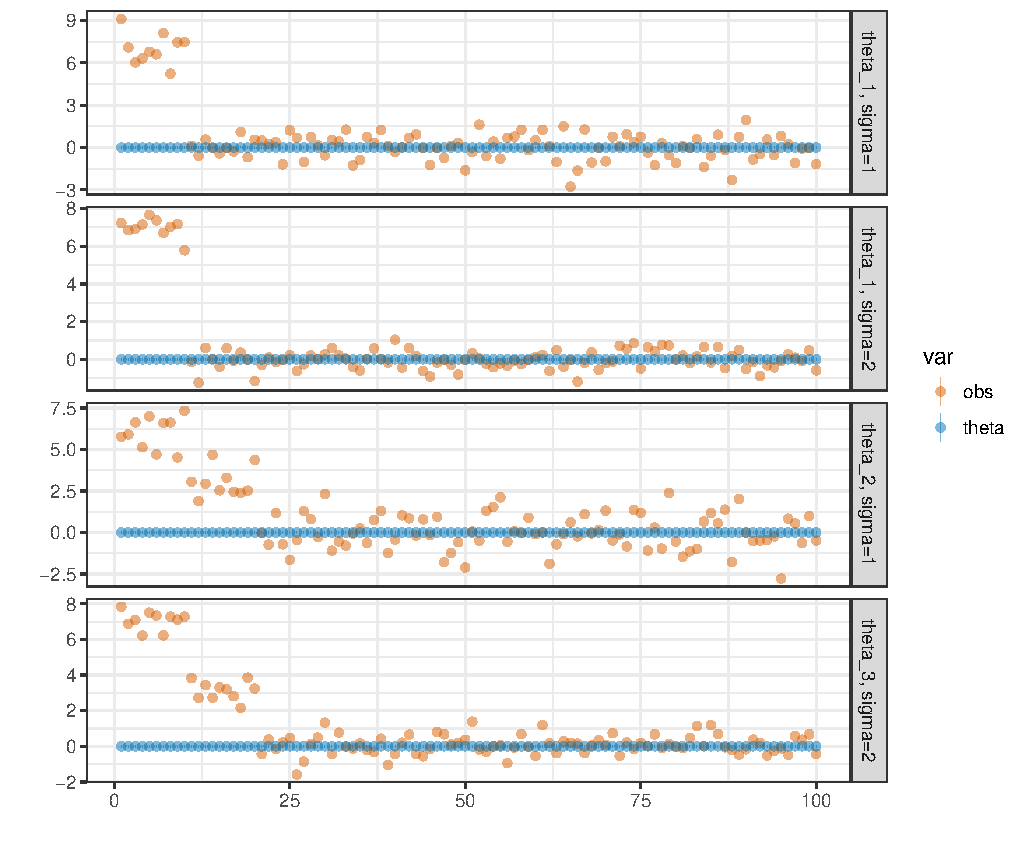
\includegraphics[width=\columnwidth]{art/sparse-means-sql-1}%
\caption{Comparison of posterior mean estimates for two different sparse normal means, $\beta_i \sim 0.8 \delta_{\{7\}}+0.1\delta_{\{3\}}+0.1\delta_{\{0\}}$ and $\beta_i \sim 0.9 \delta_{\{7\}}+0.1\delta_{\{0\}}$ under the Bayesian $\sqrt{\text{Lasso}}$ . }%
\label{fig:sql-sim-1}%
\end{figure}

The Bayesian square-root Lasso method described above has sharpened ability to detect signals in a sparse regime. We demonstrate the sparse signal recovery of the Bayesian $\sqrt{\text{Lasso}}$ through a simulation study for estimating a sparse normal mean vector for two different choices of $\bbeta$: 
\ben
\item $\bbeta = (\underbrace{7,\ldots,7}_{q_n=10},\overbrace{0,\ldots,0}^{n-q_n = 90})$ and 
\item $\bbeta = (\underbrace{7,\ldots,7}_{q_{n}=10},\underbrace{3,\ldots,3}_{r_n=10}\overbrace{0,\ldots,0}^{n-q_n-r_n = 80})$.
\een
We generate observations from a Gaussian model $(y_i \mid \beta_i) \sim \NormRV(\beta_i, \sigma^2)$ for $\sigma^2 = 1$ and $\sigma^2 = \half$. Figure \ref{fig:sql-sim-1} shows the posterior mean estimates for the four possible scenarios described above. 

%\section{Theoretical Results}
%
%\section{Future Directions}

\bibliographystyle{plainnat}
\bibliography{sqlassorefs}

\end{document}
